\section{Introducción}
En este trabajo explicaremos los conceptos teóricos de la visión artificial, su funcionamiento, su historia, las aplicaciones actuales, y los beneficios que ofrece, centrándonos en la parte del procesamiento de imágenes. 

También presentaremos un caso práctico enfocado en la detección de matrículas de coches, empleando técnicas y herramientas de procesamiento de imágenes.

\part{Conceptos teóricos}

\section{¿Qué es la visión artificial?}
La visión artificial es un campo de la inteligencia artificial que se enfoca en desarrollar métodos para que los ordenadores puedan interpretar y comprender imágenes del mundo real.

\begin{figure}[H]
    \centering
    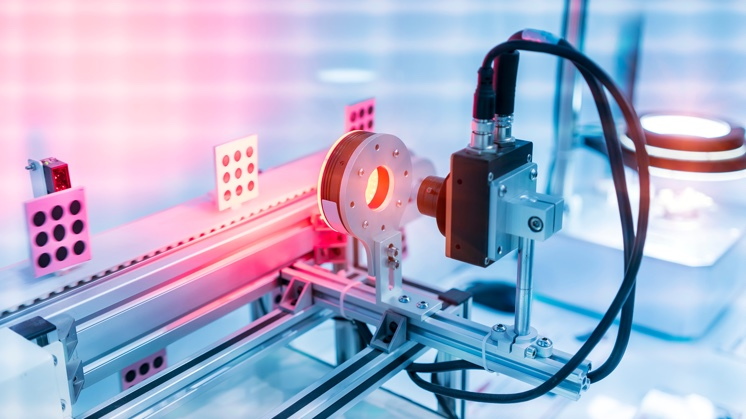
\includegraphics[width=0.5\linewidth]{Images/vision_artificial.jpg}
\end{figure}

Este campo combina técnicas de procesamiento de imágenes, aprendizaje automático y análisis de datos para permitir que las máquinas realicen tareas que simulen la visión humana. En este trabajo nos centraremos esencialmente en la parte de procesamiento de imágenes.

La visión artificial es utilizada en muchos sectores, como pueden ser: la energía, los servicios públicos, la fabricación y la automoción. El mercado de la visión artificial ha alcanzado un valor de 12,88 mil millones de dólares en 2024 y se prevé que crezca hasta los 19,21 mil millones de dólares para 2029, con una tasa de crecimiento anual compuesta del 8,3\% durante el período previsto (2024-2029) \cite{mercado}.



\section{¿Cómo funciona la visión artificial?}
La visión artificial necesita muchos datos. Se basa en ejecutar análisis de datos una y otra vez hasta que percibe diferencias y finalmente reconoce imágenes. Por ejemplo, si queremos entrenar a un ordenador para que reconozca imágenes de perros, es necesario incorporarle una gran cantidad de imágenes de perros y elementos relacionados con los perros (por ejemplo, otros animales) para que pueda aprender las diferencias y reconocer correctamente a un perro, sin confundirlo con algún otro animal.

Para conseguir esto, se utilizan dos tecnologías básicas: una especie de machine learning denominado \textit{deep learning}, y una red neuronal convolucional (CNN, convolutional neural network).

Machine learning emplea modelos basados en algoritmos que permiten a un ordenador aprender por sí solo el contexto de los datos visuales. Si se introducen suficientes datos a través del modelo, el ordenador tomará los datos y aprenderá a diferenciar una imagen de otra. Los algoritmos permiten que la máquina sea autodidacta, en lugar de que alguien la programe para que reconozca una imagen.

Una red neuronal convolucional ayuda a un modelo de deep learning o machine learning a desglosar las imágenes en píxeles a los que se asignan etiquetas. El uso de etiquetas permite realizar convoluciones y predicciones sobre lo que el ordenador está observando. Además, la red neuronal realiza convoluciones y comprueba la exactitud de sus predicciones en una serie de pasos hasta que las predicciones comienzan a pasar en el mundo real. Una vez conseguido esto, el ordenador puede reconocer imágenes de una manera similar a los humanos.


De forma parecida a un humano viendo una imagen a cierta distancia, una red neuronal convolucional primero distingue los bordes más marcados y las formas simples, luego rellena la información a medida que ejecuta iteraciones de sus predicciones. Una CNN se utiliza para comprender imágenes individuales. Una red neuronal recurrente (RNN, recurrent neural network) se emplea de manera similar en aplicaciones de vídeo para ayudar a los ordenadores a comprender cómo se relacionan entre sí las imágenes en una serie de fotogramas.

\newpage
\section{La historia de la visión artificial}

Los ingenieros y científicos de todo el mundo llevan más de 60 años intentando desarrollar formas para que las máquinas sean capaces de comprender y ver datos visuales. La experimentación dio inicio en 1959 cuando un grupo de neurofisiólogos estaban mostrando a un gato una serie de imágenes, intentando asociar una respuesta en su cerebro. Llegaron a la conclusión de que el gato respondía primero a las líneas o los bordes más marcados, lo cual significada que el procesamiento de imágenes comienza con lo más simple, las formas, como los bordes rectos. \cite{historia}

Al mismo tiempo, se desarrolló la primera tecnología capaz de escanear imágenes, permitiendo a los ordenadores digitalizar y adquirir dichas imágenes. Otro hito importante que se alcanzó en 1963 fue cuando los ordenadores fueron capaces de transformar imágenes de dos dimensiones en formas tridimensionales. En los años 60, la IA apareció como un campo académico de estudio y también marcó el inicio de la búsqueda de la IA para resolver el problema de la visión humana.

El año 1974 fue testigo de la aparición de la tecnología de reconocimiento óptico de caracteres (más conocida como OCR), capaz de reconocer texto impreso en cualquier tipo de letra o fuente. Además, el reconocimiento inteligente de caracteres (ICR) era capaz de descifrar texto que había sido escrito a mano y digitalizarlo mediante redes neuronales. A partir de ese momento, ICR y OCR se aplican en el procesamiento de facturas y documentos, pagos móviles, traducción autómata, reconocimiento de matrículas de vehículos y otros usos comunes.

Durante el año 2000, el estudio se centró en el reconocimiento de objetos, y en 2001, surgieron las primeras aplicaciones que implementaron el reconocimiento facial en tiempo real. La normalización de cómo se anotan y etiquetan los conjuntos de datos visuales apareció poco a poco a lo largo de la década de los 2000. En 2010, se hizo público el conjunto de datos ImageNet. Este conjunto de datos contenía millones de imágenes etiquetadas en miles de clases de objetos, proporcionando una amplia base para las redes neuronales convolucionales y los modelos de deep learning que se utilizan a día de hoy. En 2012, un equipo de la Universidad de Toronto participó con una CNN en un concurso de reconocimiento de imágenes. Este modelo, llamado AlexNet, redujo el índice de errores en el reconocimiento de imágenes notablemente. Gracias a este gran avance, las tasas de error se han reducido a un porcentaje muy pequeño.

\begin{figure}[H]
    \centering
    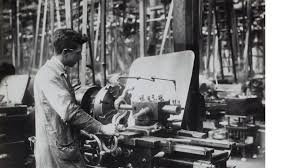
\includegraphics[width=0.5\linewidth]{Images/historia_vision_artificialjpeg.jpeg}
\end{figure}

\newpage
\section{Aplicaciones de visión artificial}
Se están realizando una gran cantidad de investigaciones en el campo de la visión artificial. Las aplicaciones del mundo real demuestran la gran importancia de la visión artificial en aplicaciones de empresa, transporte, ocio, asistencia sanitaria y tareas cotidianas. La clave para el crecimiento de estas aplicaciones radica en la gran cantidad de información visual que se genera desde cualquier dispositivo electrónico, como bien pueden ser los teléfonos móviles, cámaras de tráfico, sistemas de seguridad y cualquier otro dispositivo visualmente instrumentado. Esta cantidad de datos desempeña un papel muy significativo en distintos sectores, pero actualmente no se llegan a utilizar completamente. Gracias a toda esta información, se puede crear una base de prueba para entrenar aplicaciones de visión artificial y una plataforma de lanzamiento para que se integren en diferentes actividades humanas.

\begin{itemize}
    \item IBM empleó la visión artificial para crear My Moments y utilizarla durante el torneo de golf Masters 2018. IBM Watson vio cientos de horas de imágenes del Masters y pudo identificar tanto las escenas como los sonidos de tomas significativas. Organizó cada uno de estos momentos clave y los presentó a los seguidores como carretes personalizados de los momentos más destacados.
    \item Google Translate permite a los usuarios apuntar la cámara de un teléfono inteligente a un texto escrito en otro idioma y obtener una traducción al idioma que desee el propio usuario de una manera casi inmediata.
    \item El desarrollo de vehículos autónomos se basa en visión artificial para dar sentido a todo estímulo visual que se pueda recibir gracias a las cámaras y otros sensores del automóvil. Es crucial identificar otros vehículos, señales de tráfico, marcas de carriles, peatones, etc.
    \item IBM está utilizando la tecnología de visión artificial para aplicar la IA inteligente a edge computing y ayudar así a los fabricantes de automóviles a identificar los defectos de calidad antes de que un vehículo salga de fábrica.
\end{itemize}

\begin{figure}[H]
    \centering
    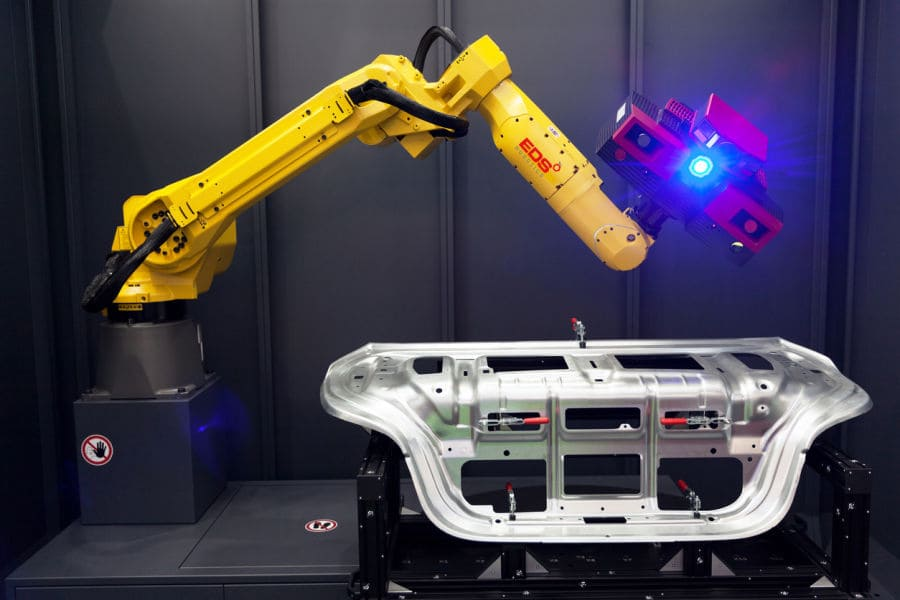
\includegraphics[width=0.5\linewidth]{Images/vision-artificial-tipos-y-aplicaciones.jpg}
    \caption{Robot de selección y de control de calidad}
\end{figure}

\newpage
\section{Beneficios de la visión artificial}
El uso de la visión artificial en empresas trae consigo numerosas ventajas, ya que no solo pueden resolver cuestiones de fabricación, sino que también pueden ayudar a mejorar la productividad. Algunos son: 

\begin{itemize}
    \item \textbf{Precisión mejorada}. Por naturaleza, las decisiones humanas se alimentan de suposiciones o ideas preconcebidas sobre la verdad. En cambio, la visión artificial basa las decisiones en datos. Además, opera a nivel de píxel, algo que el cerebro humano no es capaz de procesar. Por tanto, los resultados obtenidos son mucho más preciosos, logrando mejorar las tasas de detección de fallos hasta en un 90\%. 
    \item \textbf{Mejora en productividad}. La visión artificial puede reconocer imágenes en segundos, pudiendo destinar esos recursos humanos a tareas que requieren de la mente para ejecutarse.
    \item \textbf{Reducción de costes}. Se puede mejorar la velocidad de fabricación y reducir la mano de obra necesaria para operar el equipo. Además, puede hacer que se reduzca la cantidad de desecho, reduciendo así la cantidad de materiales empleados y, en consecuencia, una disminución de costes.
    \item \textbf{Mejora la seguridad}. La visión artificial trae consigo una reducción de participación humana, por lo que fomenta la creación de un entorno más seguro en general. Los operarios de las industrias tienden a sufrir menos lesiones y accidentes cuando operan con máquinas potentes y voluminosas. Además, se consigue que los empleados no contaminen las salas limpias y se reduce su exposición a materiales y piezas peligrosas.
\end{itemize}

Por tanto, el empleo de la visión artificial en diferentes sectores permitiría una mejora en la productividad y una reducción de costes que toda empresa busca. \cite{beneficios}




\section{Ejemplos de visión artificial}
A continuación, veremos algunos ejemplos de tareas de visión artificial establecidas:
\begin{itemize}
    \item La \textbf{clasificación de imágenes} permite ver una imagen y clasificarla (un coche, un plátano, la huella de un dedo), empleando redes neuronales convolucionales. Es más, es capaz de prever con mucha precisión que la imagen pertenece a una clase específica. Por ejemplo, una empresa de redes sociales, como puede ser Instagram, podría querer utilizarla para identificar y eliminar automáticamente imágenes censurables subidas a su plataforma por los usuarios.
    \item La \textbf{detección de objetos} puede emplear la clasificación de imágenes para relacionar una determinada clase de imagen, y luego detectar y tabular su apariencia en un vídeo o imagen. Para lograr la detección de objetos, se emplean técnicas de segmentación como las basadas en regiones, píxeles, modelos o bordes. Algunos ejemplos son la detección de daños en una línea de producción o la identificación de maquinaria que requiere mantenimiento.
    \item El \textbf{rastreo de objetos} sigue a un objeto una vez que se ha detectado. El rastreo de objetos normalmente se realiza con imágenes capturadas en secuencias o transmisiones de vídeo en tiempo real, utilizando el aprendizaje profundo o el filtro de Kalman junto a modelos de movimiento. Las cámaras de seguridad, por ejemplo, no solo tienen que clasificar y detectar personas sino que también necesitan seguirlas en movimiento para saber si acceden a zonas en las que está prohibido el acceso. \cite{rastreo}
    \item La \textbf{recuperación de imágenes basada en contenido} utiliza la visión artificial para examinar, buscar y recuperar imágenes de grandes bases de datos, en función del contenido de las imágenes en lugar de las etiquetas de metadatos asociadas. Esta tarea puede incorporar la anotación de imágenes de forma automática, en vez del etiquetado manual convencional. Además, se pueden utilizar para sistemas de activos digitales y puede mejorar la precisión de la búsqueda y la recuperación.
\end{itemize}

Algunas de las técnicas que se pueden emplear en la visión artificial y que están basadas en el procesamiento de imágenes y vídeos son las siguientes:
\begin{itemize}
    \item \textbf{Filtrado de imágenes}: La aplicación de filtros permite destacar o suavizar ciertas características de una imagen. El uso del filtro de suavizado gaussiano permite reducir el ruido de una imagen, como hemos visto durante la asignatura, mientras que el filtro de Canny es el más completo para la detección de bordes, muy usado para detectar contornos de objetos.
    \item La \textbf{transformación de imágenes} incluye operaciones como la rotación, escalado, cambio de perspectiva, etc. Gracias a estas operaciones, podemos  corregir la orientación de una imagen o ajustar su tamaño según se necesite.
    \item \textbf{Segmentación de imágenes}: podemos dividir una imagen por regiones, esto es posible gracias a la segmentación basada en un umbral, donde se clasifican los píxeles en función de su nivel de intensidad, o mediante métodos más sofisticados como la segmentación semántica, capaz de asignar una etiqueta a cada píxeles en función de su clase.
    \item \textbf{Mejora de la calidad de imágenes}: es importante trabajar con imágenes y vídeos que presenten la mayor calidad posible. Para ello, se aplican técnicas como la eliminación de ruido, la mejora del contraste y la nitidez, y la corrección del balance de blancos.
    \item La \textbf{compresión de imágenes y vídeos} permite reducir el tamaño de los archivos notablemente sin perder demasiada calidad. Se utilizan algoritmos de compresión como JPEG para imágenes y H.264, H.265, entre otros, para vídeos.
    \item La \textbf{detección de texto} en vídeos e imágenes mediante el reconocimiento óptico de caracteres (OCR) resulta muy útil. Esto es posible gracias a algoritmos de detección de objetos, que pueden detectar regiones de la imagen que contienen texto para luego segmentar y reconocer cada uno de los caracteres.
\end{itemize}

